\chapter{Defining some concepts and redefining the variables} \label{chapter:defining-some-concepts-and-redifing-the-variables}
\section{Voices, parts and strata}\label{section:parts-and-strata}
Before we start this section, we need to look at some vocabulary to make sure we understand what we are discussing. The most important definitions we introduce are the concepts of \textit{parts} and \textit{strata}. The need for these definitions arises from the increasing complexity of the rules of counterpoint when it is generalised to three voices. Indeed, the rules are no longer (as we shall see later) concerned solely with the counterpoints and the \cf, but also with new concepts, such as that referred to by Fux as 'the lowest voice'. As the term 'voice' is too generic (it is used in Fux's text to describe notions as different as 'counterpoint', '\cf', voice range and the so called 'lowest voice'), we need to create a precise vocabulary that is different from the word 'voice' to talk about these new concepts. 


With this in mind, let's explain what 'parts' and 'strata' are, and how they relate to the concept of 'voice'.

\subsubsection{Voices} Again, voices are that vague and \textit{general} concept, whereas parts and strata are more precise and \textit{specific} concepts. The concept of 'voice' includes both 'parts' and 'strata'. In other words, each of these two concepts is a type of voice. When we talk about a voice, we could be talking about either a part or a stratum. To use an object-oriented metaphor, we could say that the 'parts' and 'strata' classes inherit from the 'voice' class.

Since there are as many parts and layers as there are voices, in a composition with $n$ voices there will also be $n$ parts and $n$ layers.

\subsubsection{Parts}
Parts are an intuitive and concrete concept because each part corresponds to what a particular person sings or what a particular instrument plays. They correspond to a staff (each staff corresponds to a part). The term 'part' is the same as that used by Fux in his \gap. The three parts in a three-part composition are: the \cf, the first \cps and the second \cp. Fux distinguishes them by calling them by the name of their range, i.e. "bass", "tenor", "alto" or "soprano" (obviously you cannot have all four in a three-part composition).

\subsubsection{Strata}
As for the strata, they are defined like this: a stratum delineates discrete layers or levels of pitches at any given moment in the composition. It denotes a vertical alignment of simultaneous notes and organizes them into distinct strata. By definition, the lowest stratum encompasses the lowest sounding notes, the highest stratum comprises the highest sounding notes, and intermediary strata represent pitch levels in between.
This concept is very helpful in identifying and categorising the vertical placement of pitches, creating distinct categories of sound within the overall texture of the counterpoint composition. It provides a way of analysing and understanding the distribution of pitches across different parts, allowing more complex rules to be established. For example, it would now be possible to establish a rule between the notes of the cantus firmus and the highest sounding notes (no matter which part they come from). The full potential of strata lies in harmonic rules, but as we shall see, some melodic rules are also related to it.

\paragraph*{Important note concerning the strata}
Strata are an abstract concept, useful only in the mathematical formalisation of Fux's rules. They are necessary because we need a structure that is able to comprehend the lowest sounding note for each bar. The strata concept is obviously not needed to write counterpoint as a human being, and the aim behind its definition is not to create a new concept for music theory, but to enable us to use a tool in our constraint programming way of conceiving counterpoint composition.

\paragraph{}
\begin{wrapfigure}{r}{0.3\textwidth}
    \centering
    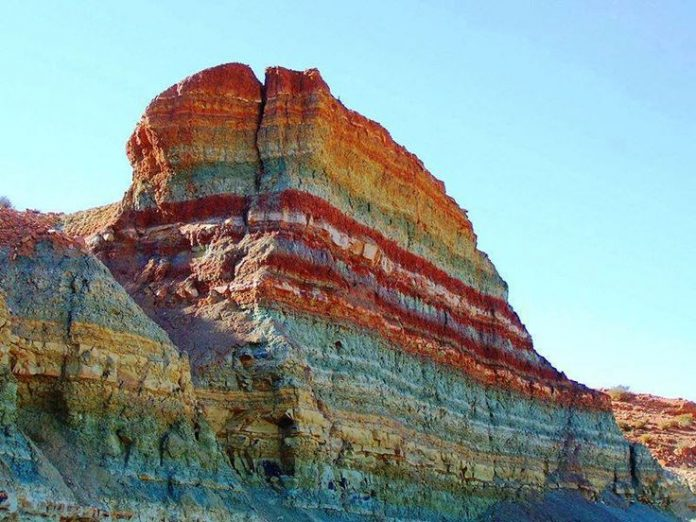
\includegraphics[width=\linewidth]{Images/rainbow-sediment.jpg}
    \caption{Geological strata, for illustration}
    \label{fig:geological-strata}
\end{wrapfigure}

The term stratum was chosen in this context for its visual impact. In geology, a 'stratum' "is a rock layer with a lithology (texture, color, grain size, composition, fossils, etc.) different from the adjacent ones"~\cite{mcnair2023}, see figure~\ref{fig:geological-strata}.
\paragraph{}
When Fux speaks about the lowest stratum, he often uses the word 'bass'. It was deliberately chosen to speak about the 'lowest stratum' instead of the 'bass' (like Fux does), because 'bass' is also the name of a range of voices (like soprano and alto, for example), and there is already enough complexity in all the terminology to add even further ambiguity.

These new terms (parts and strata) are used where the distinction between the concepts is important. Whenever this distinction is not relevant, the more general term 'voice' is used to reduce the complexity of reading. In this case, the 'voice' could refer to either a stratum or a part. And since a picture is worth a thousand words, Figure~\ref{fig:lowest} illustrates the difference between parts (the blue lines) and strata (the red and orange lines). The lowest stratum is shown in its own colour (red) because it is the most meaningful stratum, and it is particularly important in the formalisation.

\begin{figure}[h]
  \centering
  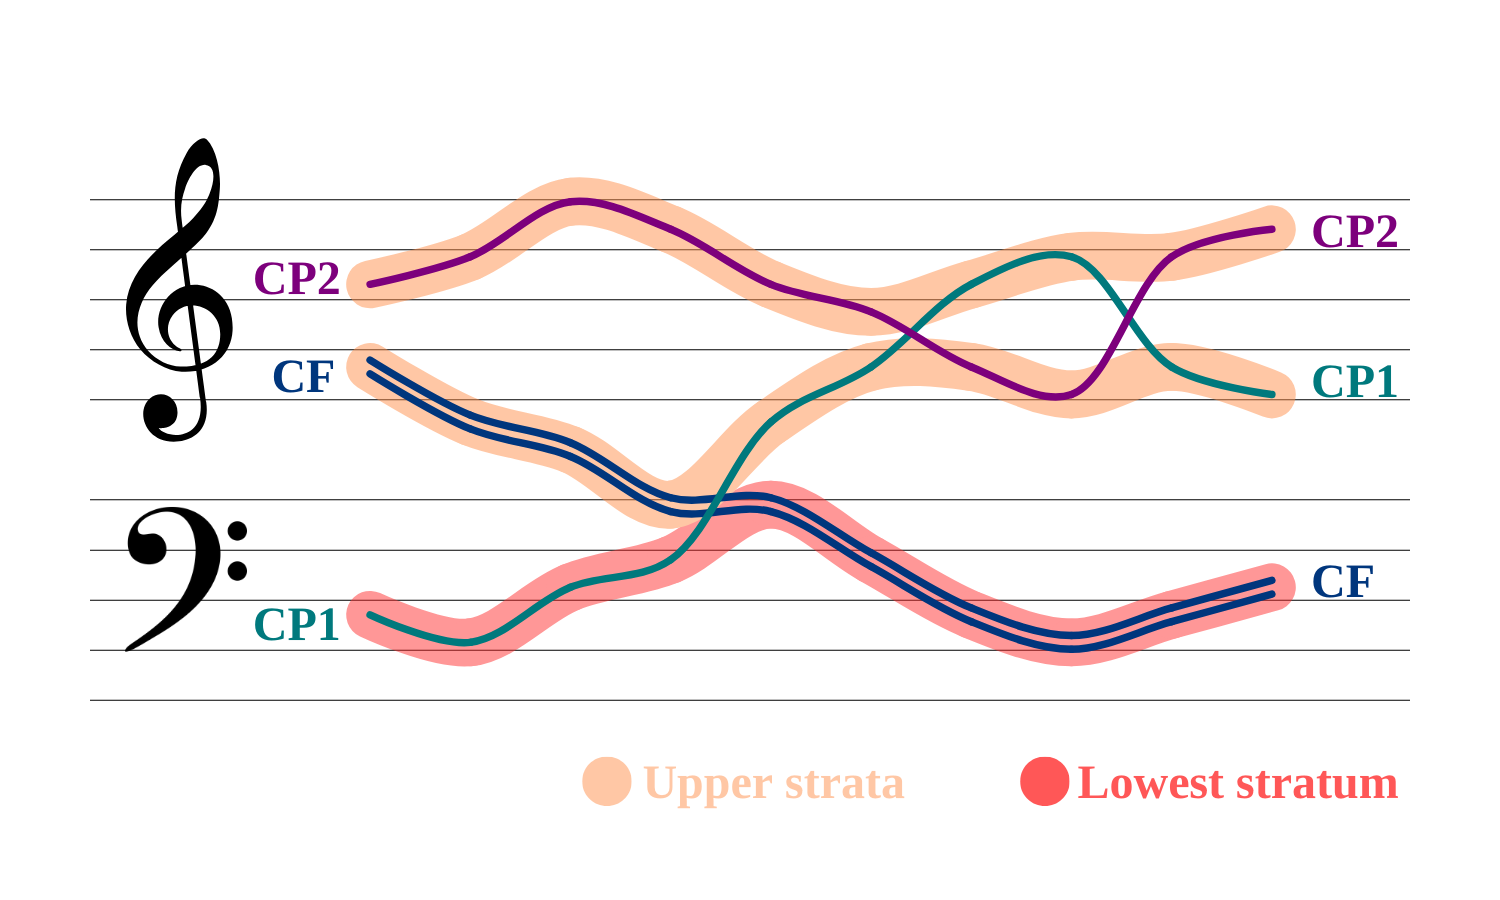
\includegraphics[width=1\textwidth]{Images/strata_example.png}
  \caption{Parts and strata in a three voice composition}
  \label{fig:lowest}
\end{figure}

\paragraph{}
Here is also the mathematical representation for the notes of the lowest stratum (written $N(a)$, see section~\ref{section:changes induced} for the notations):
% todo a, b, c, et A
\begin{equation}
    \forall i \in [0, 3] \quad \forall j \in [0, m-1): N(a)[i,j] = \text{min} (N(\mathit{cf})[i,j], N(cp_1)[i,j], N(cp_2)[i,j])
\end{equation}

The first upper stratum, or medium stratum (written $N(b)$, see section~\ref{section:changes induced} for the notations):
\begin{equation}
    \forall i \in [0, 3] \quad \forall j \in [0, m-1): N(b)[i,j] = \text{med}\footnote{Where $\text{med}(X)$ means the median value of X.} (N(\mathit{cf})[i,j], N(cp_1)[i,j], N(cp_2)[i,j])
\end{equation}

The second upper stratum, or uppermost stratum (written $N(c)$, see section~\ref{section:changes induced} for the notations):
\begin{equation}
    \forall i \in [0, 3] \quad \forall j \in [0, m-1): N(c)[i,j] = \text{max} (N(\mathit{cf})[i,j], N(cp_1)[i,j], N(cp_2)[i,j])
\end{equation}

\subsubsection{One part per stratum and one stratum per part} \label{subsubsection:one-part-per-stratum}
It is important to note that, for each musical measure, there is a bijection between the individual parts and the corresponding strata. This means that, for any given measure, each stratum uniquely corresponds to a single part, and vice versa. Put differently, if two parts within a measure share the same pitch, they do not constitute the same stratum. Instead, one part corresponds with one stratum, and the other one to a separate stratum.

To illustrate this, consider a scenario in a two-voice composition (see figure~\ref{fig:one-voice-max-can-be-a}), where part 'cf' and part 'cp1' in measure X both have a pitch value of 67 (representing a G). Despite having identical pitches at the same moment, one part is categorised as the lowest stratum, while the other is designated as the uppermost stratum. This distinction becomes crucial for subsequent analysis, especially when calculating aspects like motions.

To know which part gets to be the lowest stratum in such situations, an arbitrary hierarchical rule is implemented. If the ambivalence is between the \cfs and another part, the \cfs is always prioritised and assigned the role of the lowest stratum, over any other part. In the case of a ambivalence between the first \cps and the second \cp, the first \cps is given the status of the lowest stratum. 

\begin{figure}[h]
    \centering
    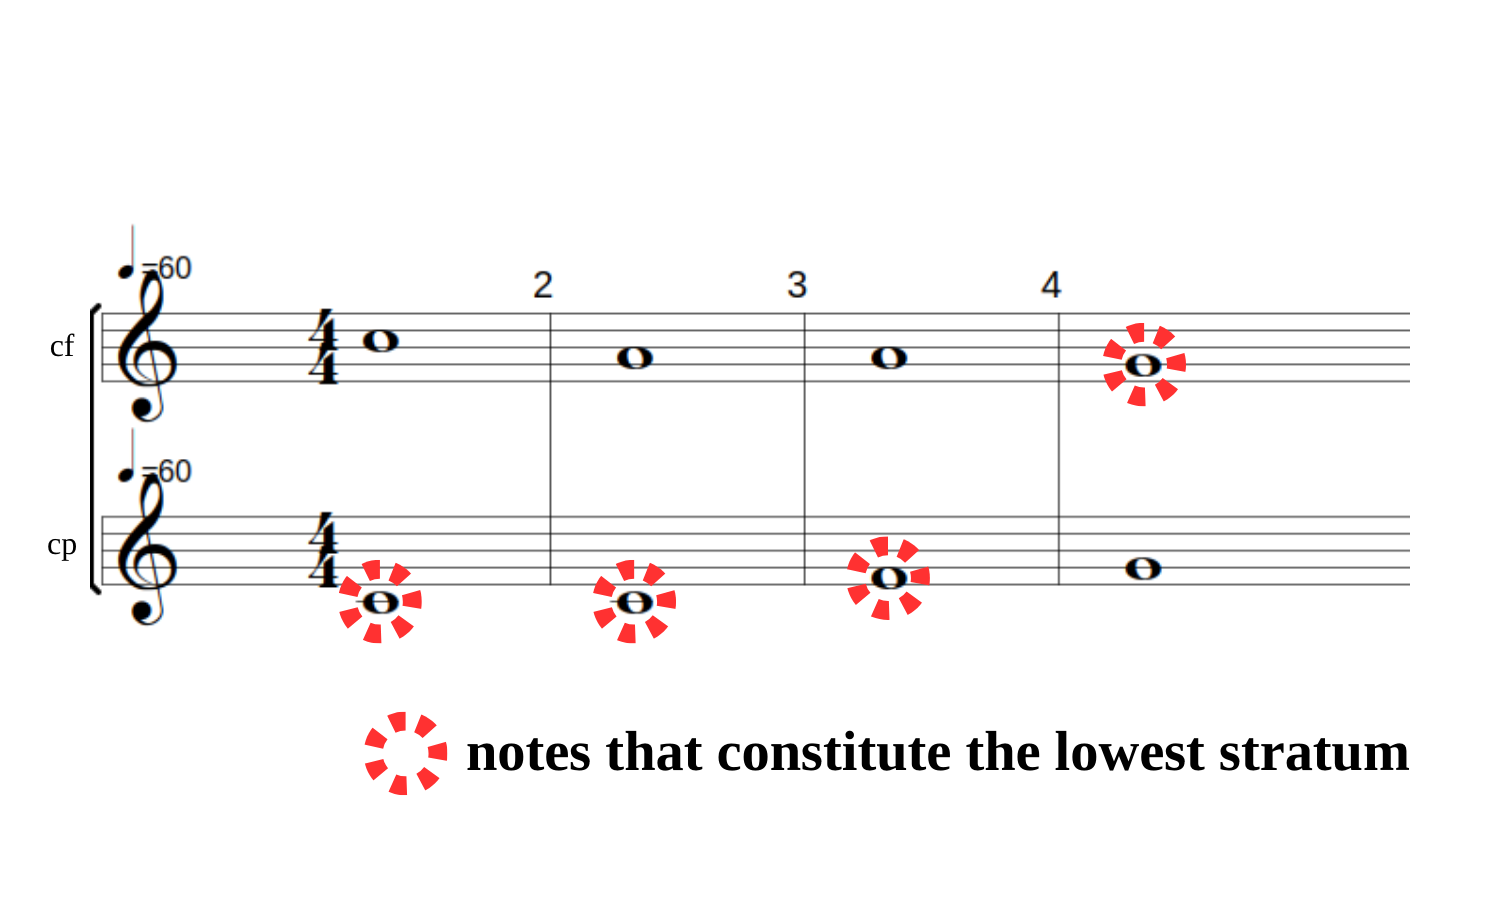
\includegraphics[width=.5\textwidth]{Images/one-voice-max-can-be-a.png}
    \caption{Establishing which part corresponds to the lowest stratum}
    \label{fig:one-voice-max-can-be-a}
  \end{figure}

\subsubsection{Note concerning the intersection of the voices}
This new stratum concept makes it possible to create compositions in which the bass doesn't always play the lowest notes, and this is precisely its purpose. Note, however, that in order for a voice other than the bass (the tenor, for example) to play the lowest note, the melodies of the tenor and the bass must cross. Fux is strangely silent on this subject: he says that crossings are perfectly permissible, but he doesn't elaborate. Other authors are clearer, and the rules of species counterpoint generally state that crossing is allowed, but that the voices must not remain inverted for too long~\cite[p.28]{Bitsch}. However, this is a rule that was not taken into account in the formalisation because it is not present in \gap. It is therefore a way of improving the FuxCP tool, with the aim of making it compatible with other styles of counterpoint.

\section{Exploring the interaction of the parts with the lowest stratum} \label{exploring-interaction-p-a}

One of the major differences between the composition of two voices (i.e., one \cfs and one counterpoint) and the generalisation to three voices (i.e., one \cfs and two counterpoints) is that the rules no longer necessarily apply between the counterpoints and the \cf, but instead of this are mostly applied \textbf{between the different parts and the lowest stratum}. 

If we go back to the rules for two voices, we see that each of them applied between the single counterpoint and the \cf. For example, when it was stated that each interval must be consonant, this referred to the harmonic interval between the counterpoint and the \cf.
On the other hand, in his second part (where he describes the rules for composing in three voices), Fux explains that the rules do not necessarily have to be followed between each counterpoint and the \cf, but rather between "each of the voices and the lowest voice" (i.e. the lowest stratum). Again, if we take the example of the need for consonance between the voices, consonance will be required in the intervals between the notes of any voice and those of the lowest voice (whether or not the latter is the \cf).
Fux approaches the concept of lowest stratum without ever stating it clearly, mentioning for example that the lowest voice can change (sometimes the bass is the lowest voice, sometimes the tenor, ...), and that at any given moment the lowest voice should be considered. In other words, Fux says that the rules apply between the parts and the lowest stratum.

In summary, the constraints are as follows:
\begin{itemize}
    \item Most of the constraints apply:
    \begin{itemize}
        \item Between the \cfs and the lowest stratum.
        \item Between the first \cps and the lowest stratum.
        \item Between the second \cps and the lowest stratum.
    \end{itemize}
    \item Some constraints apply:
    \begin{itemize}
        \item Between the \cfs and the first \cp.
        \item Between the \cfs and the second \cp.
        \item Between the first \cps and the second \cp.
        \item Between the three parts altogether (harmonic rules only).
    \end{itemize}

\end{itemize}


\subsubsection{Generalisation of two-voice counterpoint}
One might be tempted to conclude that three-part composition breaks completely with two-part composition, but that would be too hasty a conclusion. Indeed, on closer inspection, the way the rules worked in two-part composition (from counterpoint to \textit{cantus firmus}) is just one particular case of this new vision of things. In two-part composition, too, the rules apply between the parts and the lowest stratum. But of course, since there were only two voices, the lowest stratum was either counterpoint or cantus firmus. This means that when links were established between the upper part and the lowest stratum, links were also established between the counterpoint and the cantus firmus. Considering the rules as being established between the counterpoint and the \cfs was just a simplification of reality, although it was perfectly correct. We were therefore considering a convenient particular case, and not the general case. Please note that when we talk about "applying constraints from voice A to voice B", it is clear that the constraints are bidirectional and that they also apply from voice B to voice A. What is shown here is rather the philosophy behind the application of these constraints, and the reasons why they were imposed.

The particular case happening when composing with two parts is illustrated in figures~\ref{fig:cp2cf-2v} and~\ref{fig:p2l-2v}. As we can see on those pseudo-compositions, it does not change anything to apply the constraints between the counterpoints and the \cfs or between the parts and the lowest stratum.

\vspace{.5cm}
\begin{minipage}{0.46\textwidth}
    \centering
    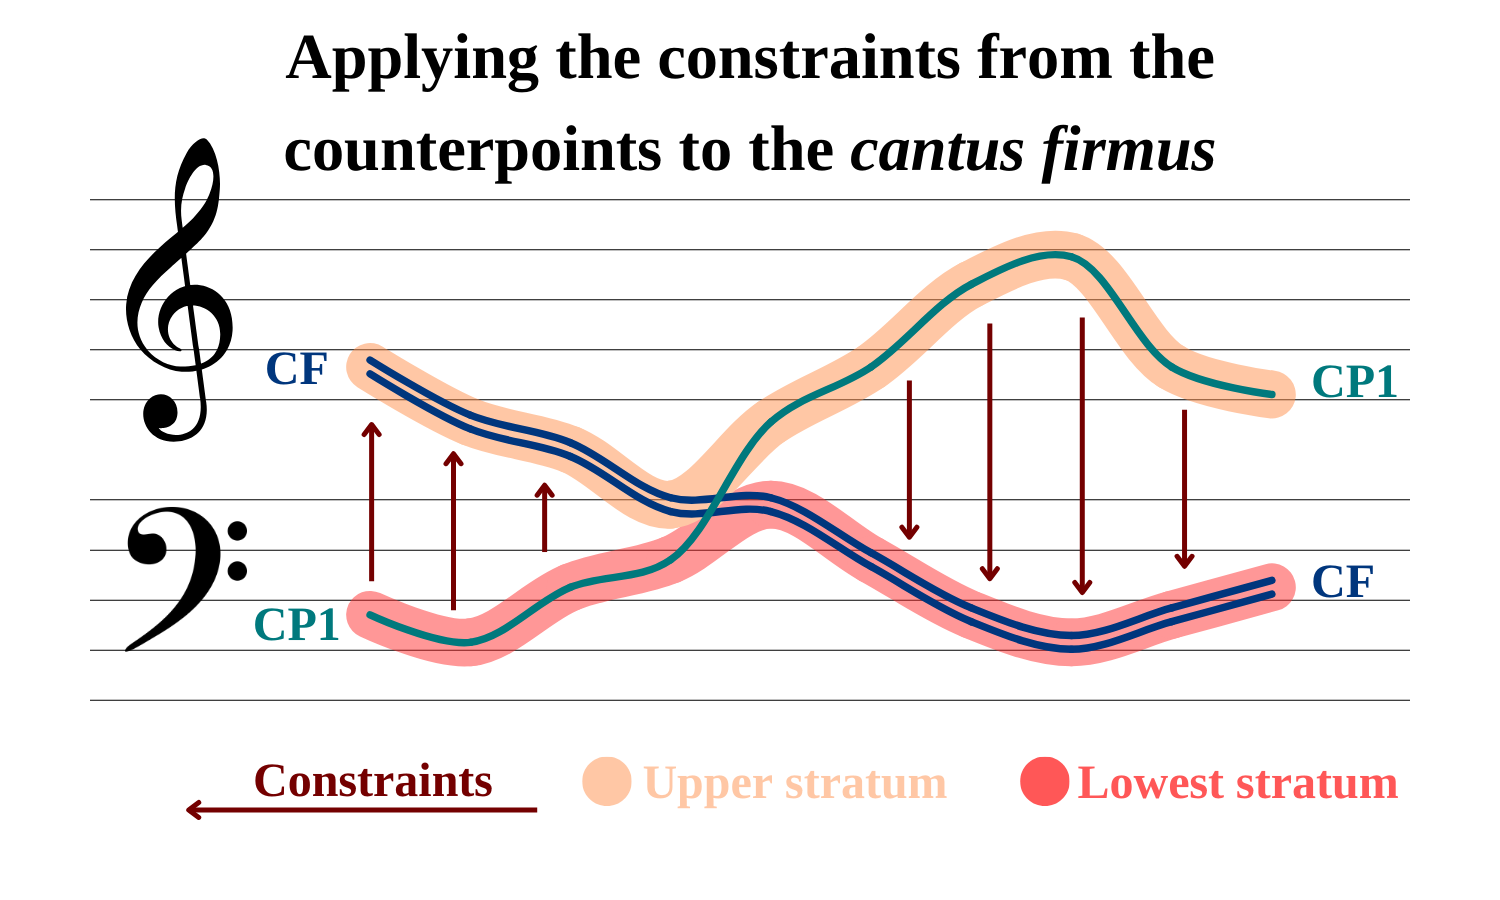
\includegraphics[width=\textwidth]{Images/cp2cf-2v.png}
    \captionof{figure}{Applying the constraints between the counterpoint and the \cf}
    \label{fig:cp2cf-2v}
    \end{minipage}
    \hfill
    \begin{minipage}{0.46\textwidth}
      \centering
      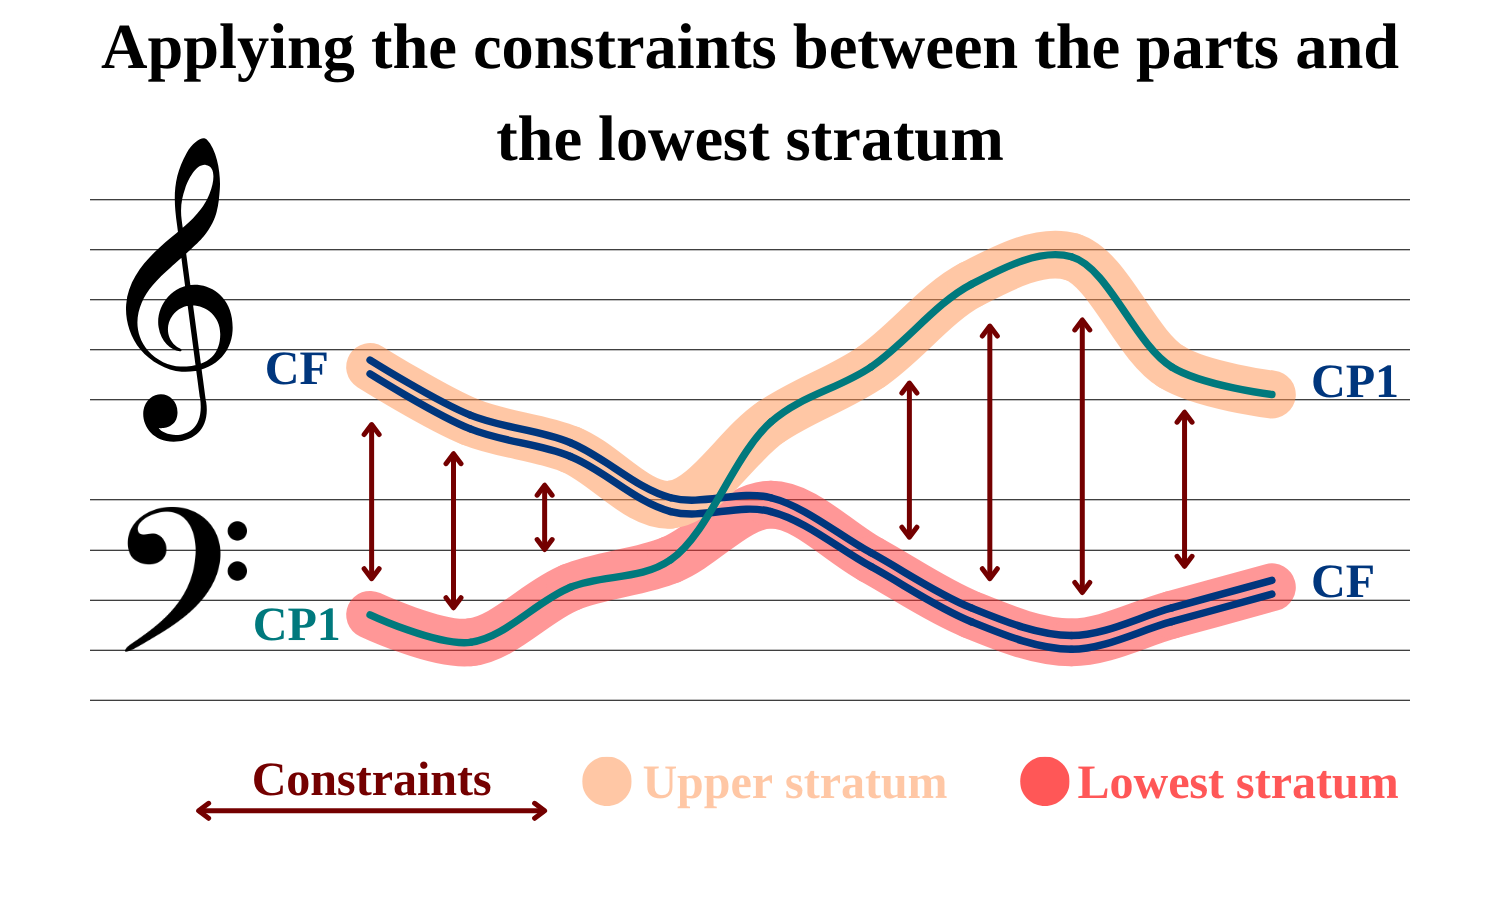
\includegraphics[width=\textwidth]{Images/p2l-2v.png}
      \captionof{figure}{Applying the constraints between the parts and the lowest stratum~~~~~~~}
      \label{fig:p2l-2v}
\end{minipage}
\vspace{.5cm}

However, when it comes to generalising the composition of counterpoint for three voices, the same simplification is no longer possible. We are now forced to establish our rules between the parts and the lowest stratum, and no longer between the counterpoints and the \cf. In figures~\ref{fig:cp2cf-3v} and~\ref{fig:p2l-3v} it becomes clear that establishing the rules between the counterpoints and the \cfs is really different from applying them between the various parts to the lowest stratum. In these figures, the parts don't intersect and therefore fit perfectly with the strata, so the constraints are always applied to the same counterpoint. This was done for the sake of intelligibility of the graphs, but it is of course possible for the parts to cross and for the "target" of the constraints not always to be the same counterpoint.

\vspace{.5cm}
\begin{minipage}{0.46\textwidth}
    \centering
    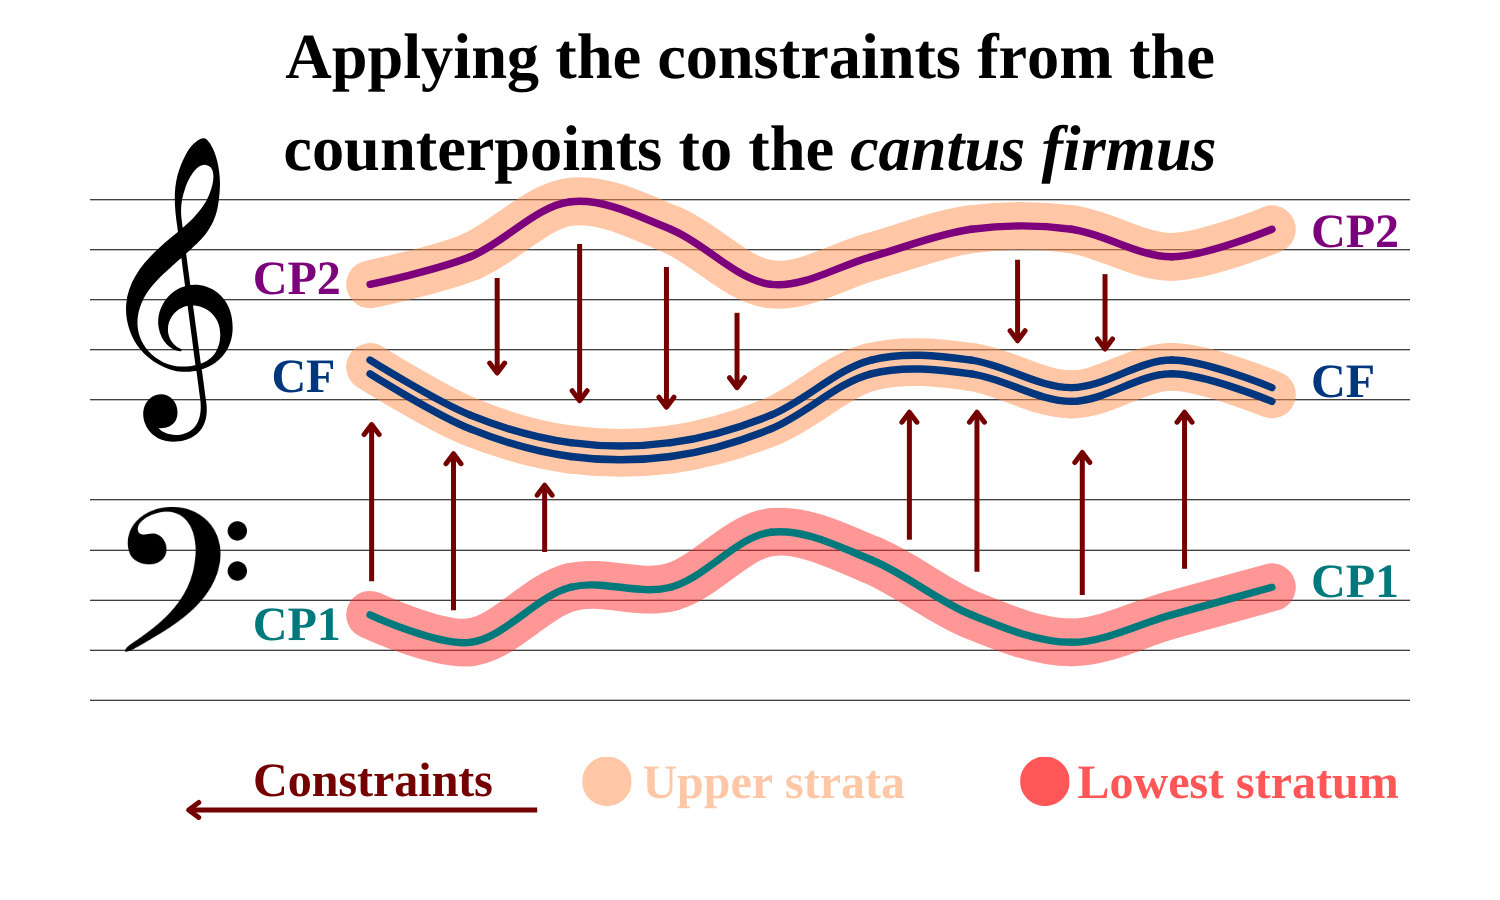
\includegraphics[width=\textwidth]{Images/cp2cf-3v.png}
    \captionof{figure}{Wrong approach: applying the constraints between the \cps to the \cf.}
    \label{fig:cp2cf-3v}
    \end{minipage}
    \hfill
    \begin{minipage}{0.46\textwidth}
      \centering
      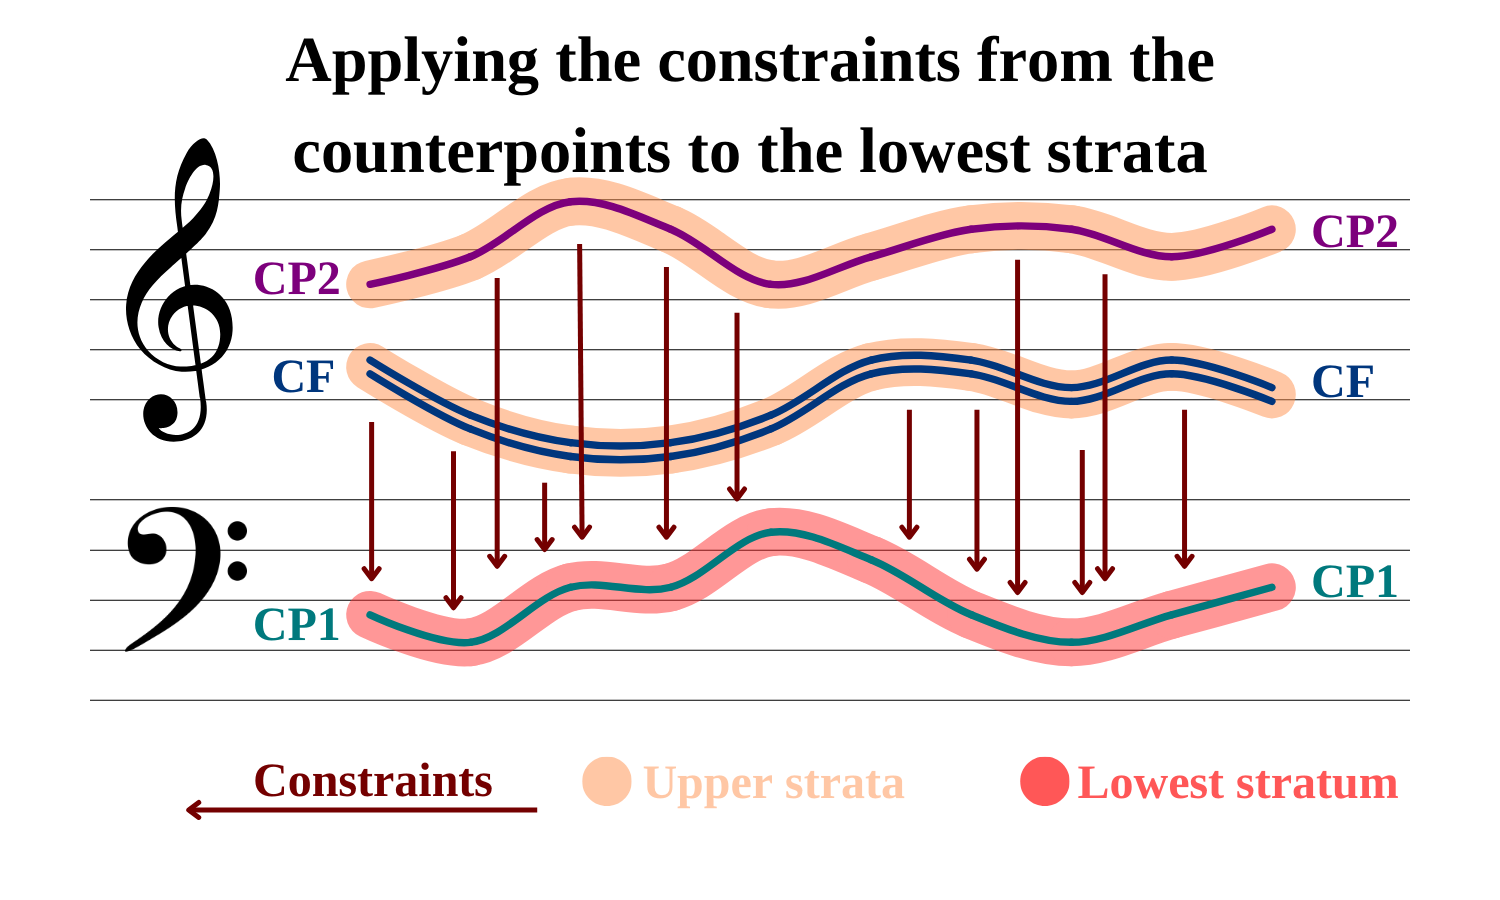
\includegraphics[width=\textwidth]{Images/p2l-3v.png}
      \captionof{figure}{Correct approach: applying the constraints between the parts to the lowest stratum.}
      \label{fig:p2l-3v}
\end{minipage}
\vspace{.5cm}

It is, of course, possible for the \cfs to be equal to the lowest stratum all along, in which case nothing changes from the perspective we had when composing for two voices. In this particular case, by applying the rules with respect to the \cf, we would find ourselves de facto applying the rules with respect to the lowest stratum (and we would be back to the situation described above, see figures~\ref{fig:cp2cf-3v} and~\ref{fig:p2l-3v}, only that there is now one more part). It is when the \cfs pitches are higher up than those of the counterpoints that considering the lowest stratum consideration becomes necessary.

\paragraph{}
A very important detail, and perhaps the biggest change brought about by this paradigm shift, is the following. Previously, we applied constraints between the counterpoints and the \cf, which guaranteed that the \cfs was taken into account in the constraints. But if we now apply the constraints only between the counterpoints and the lowest stratum, there is no longer any guarantee that the \cfs will be linked to the other voices by any constraints, for example if the \cfs is not the lowest stratum. Nevertheless, it is important that the relationship between the \cfs and the lowest stratum is \textit{also} taken into account, not just the relationship between the counterpoints and the lowest stratum. This means that when we apply the constraints between the parts and the lowest stratum, we \textit{must} also apply them to the \cfs (since the \cfs is a part, like any of the counterpoints), unless explicitly stated otherwise. 

A second point to bear in mind, and not the least, is that all this does not mean that \textit{all} the rules are established between the parts and the lowest stratum. Certain rules continue to apply between the different parts, regardless of whether they are high, low or intermediate.

\section{Definitions of the variables used in the formalisation} \label{section:changes induced}
In this section we define the variables used in the formalisation. Many of these variables were already present in T. Wafflard's work and are reused in this formalisation, with some changes. All these (re)definitions are explained in detail in this section.

Throughout this section, when reference is made to the past ("this variable used to be", "this variable keeps the same definition", ...), it means that reference is made to the previous definition of the variable, which was the one defined in T. Wafflard's work.

\paragraph{Nota bene}
Please take into consideration that all the rules from T. Wafflard's thesis (which can be found in Appendix~\ref{appendix:complete-set-of-rule}) are fully compatible with the new definitions of the variables, as discussed in~\ref{exploring-interaction-p-a}. 

%TODO
\subsection{Variables and array notation} \label{Wafflard-variables}
First, let's look at how the variables are defined and the notation we use to access them. The variables are defined to capture a compositional reality, such as the notes of the voices, the harmonic intervals between those voices, or many other concepts. They are represented by a letter ($N$ for the notes, $H$ for the harmonic intervals, ...) and are mainly arrays because they have a different value for each beat of the composition. To know which beat we are talking about, we address the variable in a computer notation. For example, N[i, j] means "the note on the i-th beat of the j-th measure". This implies that $i$ ranges from $0$ to $3$ and that $j$ ranges from $0$ to the number of measures (which is written as $m$).

Once defined, the variables are related to each other according to the formalised rules. The constraint solver searches for all possible values of these variables, according to the constraints, and stops when all variables in $N$ (the pitches) are fixed, as this means that a solution has been reached (the notes of the counterpoints are known, and this is the goal of the solver).

Of course, there are many different solutions for the same \cf, and in order to distinguish between two valid solutions (i.e. all solutions that respect all constraints). So some variables are actually costs, that are intended to convey the preferences expressed by Fux in \gap. Thus, the solver considers a valid solution with a low cost to be better than a valid solution with a high cost. The costs can be $0$ (no cost), $1$ (low cost), $2$ (medium cost), $4$ (high cost), $8$ (last resort) and $64m$ (cost proportional to length). These costs are then combined into a total cost that the solver tries to minimise. We will see in chapter \ref{chapter:search} how the costs are actually combined.


\subsection{Overview of all the variables}
We may now take a look at all the variables that are useful throughout this work. You may note that a vast majority of them already exists in T. Wafflard's thesis, but with one big change, each variable is now linked to a voice. To understand this, let's take an example. In a two-part composition, it was obvious that H (the harmonic intervals array) described the intervals between the \cfs and the only counterpoint. It was also obvious that P (the motions array) described the motions of the single counterpoint. And so it is with all the variables. When writing a three-voice composition, we have many possibilities when we talk about intervals or motions. Intervals between which voices? Movements of which counterpoint? To deal with this, each variable is now related to a voice.

The relationship between a variable and a voice is expressed as a function. $X(v)$ represents the variable $X$ of the voice $v$. The arguments of the function can be either:
\begin{itemize}
    \item $\mathit{cf}$ - for linking the variable to the \cf.
    \item $cp_1$ - for linking the variable to the second \cp.
    \item $cp_2$ - for linking the variable to the third \cp.
    \item $a$ - for linking the variable to the lowest stratum.
    \item $b$ - for linking the variable to the intermediate stratum.
    \item $c$ - for linking the variable to the uppermost stratum.
  \end{itemize}

\noindent For example, $X(\mathit{cf})$ refers to the variable $X$ of the \cf.

\paragraph{}
When a variable is not explicitly linked to a voice, it is implied that the relation expressed for it is true for all \textit{parts}. In other words, if the variable $X$ is written without any precision, it means that we are speaking about the variable X of all parts. Formally, $X \equiv \forall v \in \{\mathit{cf}, cp_1, cp_2\}: X(v)$. This is very important, as it makes it possible for T. Wafflard's rules for two voices to \textit{remain valid} even with the new definition of the variables.

\paragraph{}
\noindent As mentioned before, linking the variables and the voices is something that applies to all variables, namely\footnote{This list contains all the variables used in this thesis and a short description of them. All variables are defined accordingly, even the ones from T. Wafflard's thesis. However, the explanation of these reused variables is less detailed than in T. Wafflard's thesis: for more information on them, please refer to his work.}:
\begin{itemize}
    \item \textbf{N}(v) - the notes (pitches) of the voice v. This is the same variable as the variable 'cp' in T. Wafflard's thesis.
    \item \textbf{H}(v$_1$, v$_2$) - the harmonic intervals between voice v$_1$ and voice v$_2$. This variable is particular, as it needs two arguments to be meaningful.
    \item \textbf{M}(v) - the melodic intervals of the voice v, 
    \item \textbf{P}(p) - the motions of the part p,
    \item \textbf{A}(p) - the boolean array representing whether the part p is the lowest stratum.
    \item \textbf{IsCfB}(v) - the boolean array representing whether the cantus firmus is lower than the voice v,
    \item \textbf{IsCons}(v) - to the boolean array representing whether the voice v is consonant with the lowest stratum or not,
    \item \textbf{S}(p) - an array specific to the fifth species, representing for each beat what set of rules a note follows. For example $S[0, 0]=3$ means that the very first note of the fifth species counterpoint actually belongs to the third species. This is important since the fifth species is actually a mixture of all the others.
\end{itemize}

\noindent It also applies to \textit{some} constants, namely:
\begin{itemize}
    \item \textbf{species}(p) - the species of part p --- by definition, $species(\mathit{cf}) = 0$,
    \item \textbf{n}(p) - the number of notes in part p,
    \item \textbf{s$_\text{m}$}(p) - the maximum number of notes contained in part p, if all notes were quarter notes, excepted the last one (that is always a whole note),
    \item \textbf{lb}(p) - the lower bound of the range of part p,
    \item \textbf{ub}(p) - the upper bound of the range of part p,
    \item $\mathcal{R}$(p) - the range of part p, i.e. $\mathcal{R}(p) := [lb(p), ub(p)]$,
    \item \textbf{borrow}(p) - the borrowing scale\footnote{Remember that Fux mainly uses notes without a flat or sharp, which means that if the composition begins with a C, it will be written in Ionian mode, if it begins with a G, in Mixolydian mode, etc. Borrowing mode is a way for counterpoint to access notes that are not originally in its mode. For example, a counterpoint in E (i.e. Phrygian mode) that has the major mode (E major, i.e. Ionian E) as its borrowing mode will also have access to the notes F\#, C\#, G\# and D\#.} of part p,
    \item $\mathcal{N}$(p) - the borrowed notes of part p, where $\mathcal{N}^{\mathcal{R}}(p) = \mathcal{N} \cap \mathcal{R}$
    \item $\mathcal{B}$(p) - the set of beats\footnote{To make it clearer: for the first species, the only beat in a measure is $\{0\}$, as there is only a note on the first beat. For the second species, the set of beats is $\{0, 2\}$. For the third species, it is: $\{0, 1, 2, 3\}$. For the fourth species: $\{0, 2\}$. And for the fifth species: $\{0, 1, 2, 3\}$.} in a measure according to the species of part p,
    \item \textbf{b}(p) - the number of beats\footnote{Thus, it is always equal to the size of the set $\mathcal{B}$(p).} in a measure according to the species of part p,
    \item \textbf{d}(p) - the duration of a note\footnote{For the first species, it is equal to $1$, as each note is a whole note. For the second species, it is $\dfrac{1}{2}$, for the third, it is $\dfrac{1}{4}$, for the fourth, it is $\dfrac{1}{2}$, and for the fifth, it is $\dfrac{1}{4}$. It is always equal to $\dfrac{1}{b(p)}$.} according to the species of part p,
    \item \textbf{m} - the number of measures in the composition, which is the same for all voices,
    \item \textbf{Dis} - the set of all consonances, i.e. $\{1, 2,5, 6, 10, 11\}$
    \item \textbf{Cons} - the set of all consonances, i.e. $\{0, 3, 4, 7, 8, 9\}$, where Cons$_p$ are the perfect consonances, i.e. $\{0, 7\}$, and Cons$_{h\_triad}$ are the consonances of a harmonic triad as defined by Fux, i.e. $\{0, 3, 4, 7\}$.
\end{itemize}
Please note that the constants can only be linked to the parts, never to a stratum. Indeed, it would have no sense to speak about the species of a stratum or about the extended domain of a stratum.

The costs are also affected by the linking, except for $\mathcal{C}$ (the cost factors) and $\tau$ (the total cost). The latter are global variables that exist only once. For a summary of all costs, please refer to Table \ref{tab:cp-params}.

\paragraph{}
To make sure that those notations are clear, here are some examples: the notation $N(a)$ corresponds to the variable representing the notes (pitches) of the lowest stratum, whereas $N(\mathit{cf})$ are the notes of the \cf. The species of the second counterpoint is written $species(cp_2)$. If only $N$ is written, then the equation in which $N$ is located holds true for any possible \textit{part}. That is, the relationship $N[0, 0] < 60$ would mean: the pitch of the first note \textit{of all parts} must be lower than a middle C (whose representation in MIDI is 60).

\subsubsection{Note regarding the fourth species}\label{nota-bene-4th-species} Let's recall that the fourth species behaves in a particular way compared to the other species. First of all, it is exclusively composed of syncopations. Its notes are half notes, always linked two by two from bar to bar, producing a pitch change in the middle of the measure, on the upbeat. This gives the impression of hearing a whole note that is constantly shifted by two beats, in other words: syncopation.

Concretely, and as Fux explains it, the syncopation means that the beats of the fourth species should be considered as "shifted": its upbeat should be considered as the downbeat, and its downbeat as the upbeat of the previous measure. This means that in the majority of cases, the equations for the fourth species would have to be rewritten, swapping the 0 and 2 indexes (H[2, j] becomes H[0, j] and H[0, j+1] becomes H[2, j]). To avoid duplicating each of the equations (a first equation if it is not of the fourth species and a second equation if it is of the fourth species) and also to avoid equations that are too complex and difficult to read, it was decided that the index swap would be implicit.

Here is an example: $H[0, 0] = 7$ should be understood as $H[2, 0] = 7$ if it concerns a fourth-species counterpoint.

\subsection{In depth definition of the variables} \label{section:definition-variables}

\noindent \textbf{N}(v) \hspace{.2cm} \texttt{notes} 

N is the array corresponding the pitches of each voice. Its size is $s_m$. It is the same array as the one named \texttt{cp} in T. Wafflard's thesis, and it got renamed to \texttt{N} (for notes), for the sake of clarity. As we have now three of those arrays (one for the first counterpoint, one for the second counterpoint, and even one for the \cf), it needed a less ambiguous name than the one it had before. 

The notes in array N are written in MIDI format. This means that a middle C ($C_4$ in scientific pitch notation) is represented by 60, and each semitone has a value of 1. So, starting from the middle C, we have:

$\{C_4, D_4, E_4, F_4, G_4, A_4, B_4\} \equiv \{60, 62, 64, 65, 67, 69, 71, 72\}$.

%\begin{equation}
%    \forall i \in \B, \forall j \in [0, m): Cp[i, j]\in \N^{\R}
%\end{equation} 



\vspace{.5cm} \noindent \textbf{H}$_{(\text{abs})}$(v$_1$, v$_2$) \hspace{.2cm} \texttt{h-intervals}\hspace{.2cm} \texttt{h-intervals-abs}\hspace{.2cm} \texttt{h-intervals-to-cf}\hspace{.2cm}  ...

This variable is an array of size $s_m$ and represents the harmonic intervals between voice v$_1$ and voice v$_2$. It is the only variable that is associated with two different voices. So $H(v1,v2)[i,j]$ represents the intervals between the $i$th beat of voice $v_1$ and the \textit{first} beat of voice $v_2$. $v_1$ can be a part and $v_2$ can be a stratum, since you can calculate harmonic intervals between a part and a stratum. If $v_2$ is not specified, it is equal to $a$ by default. In other words, $H(v_1)$ represents the intervals between the voice $v_1$ and the lowest stratum: $H(v_1) \equiv H(v_1,a)$. This default value for $v_2$ was chosen because it is the most commonly used, and for a good reason: the most relevant harmonic intervals are those between the voices and the lowest layer.

For example, here are the values of the intervals of the harmonic triad: a minor third is 3, a major third is 4, a fifth is 7 and an octave is 12 (or 0 if modulo).

\begin{equation}
\begin{aligned}
    &\forall v_1, v_2 \in \{\mathit{cf}, cp_1, cp_2, a, b, c\}, \quad \forall i \in \mathcal{B}(v_1), \quad \forall j \in [0, m):\\
    &H_{abs}(v_1,v_2)[i, j] = \left|N(v_1)[i, j] - N(v_2)[0,j]\right|\\
    &H(v_1-v_2)[i, j] = H_{abs}[i, j]\ \text{mod}\ 12\\
    &\text{where } H_{abs}[i, j] \in [0, 127], H[i, j] \in [0, 11]
\end{aligned}
\end{equation}

\vspace{.5cm}
\noindent \textbf{M}$_{\text{brut}}$(v) \hspace*{.2cm} \texttt{m-intervals-brut}

The variable M represents the melodic intervals of a voice. It can be evaluated either on a part or on a stratum, each of these situations leading to different behaviours.
\begin{itemize}
    \item 

M(p) (i.e. when related to a part) represents the melodic intervals of the part p, and its mode of operation remains the same as in T. Wafflard's thesis: M$_{brut}$[i,j] represents the melodic interval used to "leave" N[i,j]. For example, if $N[0,0]=60$ and $N[1,0]=67$, the interval used to leave $N[0,0]$ is $7$. There are several versions of this array, such as M$^x$, which represents the melodic interval between the current beat and the xth following note, according to d(p)\footnote{If d(p)=x, it means that the following note comes in x beats. So if d=1, M$^2$[0,0] represents the interval between N[0,0] and N[2,0].} and M, which represents the absolute value of M$_{brut}$. By default, $M\equiv M^1$, thus, $M\equiv \forall p \in \{\mathit{cf}, cp_1, cp_2\} \colon M^1(p)$.

\begin{equation}
    \begin{aligned}
        &\forall x \in \{1, 2\}, \forall i \in \B, \forall j \in [0, m-x) \colon \\
        &M^x_{brut}[i, j] = N[(i+xd)\ mod\ 4, j+nextm(i+xd)] - N[i, j]\\
        &M_{brut}(a)[j] = \,  
        \begin{cases}
            M_{brut}(\mathit{cf})[0][j] & \text{if } A(\mathit{cf})[j+1]\\
            M_{brut}(cp_1)[\text{max}(\mathcal{B}(cp_1))][j] & \text{if } A(cp_1)[j+1]\\
            M_{brut}(cp_2)[\text{max}(\mathcal{B}(cp_1))][j] & \text{if } A(cp_2)[j+1]\\
        \end{cases}
        &M^x[i, j] = \left|M^x_{brut}[i, j]\right|\\
        &\text{where } M^x_{brut}[i, j] \in [-12, 12], \quad M^x[i, j] \in [0, 11] 
    \end{aligned}
\end{equation}


\item M(s) (i.e. when related to a stratum) has it own way of working, that is defined in the next paragraphs. We focus specifically on M(a), the melodic intervals of the lowest stratum.
\end{itemize}

\paragraph{Why is it complicated to consider melodic intervals of strata?}
Since strata don't have melodic intervals \textit{per se} (they actually do have melodic intervals, but it doesn't really make sense to consider them), we need to redefine what we mean when speaking about the melodic intervals of a stratum. If it is not clear why strata have no inherent melodic intervals, remember that strata are an abstract concept that is used only in mathematical relationships (and respective constraints). People who listen to the music hear the different parts (be they different tessitura, different instruments, ...) and the way these parts interact together in melodic movements and harmonic convergences, rendering a beautiful music, or not. Strata are an abstraction of the harmonic interactions between the parts, and because of this, they are a consequence of the parts: they exist because the parts exist, and not the other way round! And since they are defined according to harmonic principles (as was suggested before, they are successions of vertical alignments), speaking about the proper \textit{melodic} intervals of a stratum makes no sense. One could then conclude that melodic intervals do not apply to strata, and go ahead. Nevertheless, Fux \textit{does} speak about computing the motions between a part and the lowest stratum. And to be able to compute motions, one needs to compare two different melodic intervals. So we need to have a definition for the melodic intervals of a stratum. 

\paragraph{Definition of M(s), the melodic intervals of a stratum}
To understand how we arrive at a definition for the melodic intervals of a layer, we need to remember that the lowest layer is just the collection of all the lowest-sounding notes in the composition. It is therefore quite logical to think of the melodic intervals of the lowest layer as the melodic intervals that lead to all those lowest-sounding notes. We thus define the melodic intervals of the lowest stratum to be: the interval that lead to the note of the lowest stratum in the corresponding part. Let's make this clearer with an example. Let's consider that the lowest stratum consists of the notes [C$_{cp_1}$, E$_{\mathit{cf}}$, G$_{cp_2}$] (where C$_{cp_1}$ indicates that the C belongs to the first \cp), that in the \cfs the interval that lead to the E is a +0 (i.e. staying on the same note), and that in the second \cps the interval that lead to the G was a -4 (getting down of two tones). The corresponding melodic intervals array of the lowest stratum would then be [+0, -2]. This example has been written again in a more visual way in equation~\ref{eq:defining-m-intervals-bass} to make it easier to understand. To the left of the equation is the pitch array of each voice mentioned. To the right of the equation is the melodic interval array of each voice mentioned. The numbers in bold red are those corresponding to the lowest stratum.


\begin{equation}
    \begin{aligned}        
    N(\mathit{cf}) &= [64,\quad  \textcolor{darkred}{\textbf{64}},\quad  71] \quad 
    &M_{brut}(\mathit{cf}) &= [\textcolor{darkred}{\textbf{+0}}, \quad +7]\\
    N(cp_1) &= [\textcolor{darkred}{\textbf{60}},\quad  67,\quad  74] \quad 
    &M_{brut}(cp_2) &= [+7, \quad +7]\\
    N(cp_2) &= [72,\quad  71,\quad  \textcolor{darkred}{\textbf{67}}] \quad 
    &M_{brut}(cp_2) &= [-1, \quad \textcolor{darkred}{\textbf{-4}}]\\
    \\
    N(a) &= [\textcolor{darkred}{\textbf{60}},\quad  \textcolor{darkred}{\textbf{64}},\quad  \textcolor{darkred}{\textbf{67}}] \quad 
    &M_{brut}(a) &= [\textcolor{darkred}{\textbf{+0}}, \quad \textcolor{darkred}{\textbf{-4}}]\\
\end{aligned}
\label{eq:defining-m-intervals-bass}
\end{equation}


The formal definition of the melodic intervals of the lowest stratum is hence as follows: the melodic interval in measure $j$ of the lowest stratum is equal to the last melodic interval in measure $j$ of the part that is the lowest stratum in measure $j+1$. Remember that this complex definition is needed in order for the computation of the motions to work fine, and that the motions of the lowest stratum, juste as the lowest stratum, are an abstract notion that serves only in formulas and constraints. The motions of the lowest stratum \textit{do not intend to represent any concrete motion really happening in the composition, nor does it correspond to the melodic intervals between the pitches of the lowest stratum}.It may be worth noting that if a part is the lowest stratum all the time, then the motions of the lowest stratum will be completely equal to those of that part.

\begin{equation}
    \begin{aligned}
        &\forall j \in [0, m-1):\\
        &M_{brut}(a)[j] = \,  
        \begin{cases}
            M_{brut}(\mathit{cf})[0][j] & \text{if } A(\mathit{cf})[j+1]\\
            M_{brut}(cp_1)[\text{max}(\mathcal{B}(cp_1))][j] & \text{if } A(cp_1)[j+1]\\
            M_{brut}(cp_2)[\text{max}(\mathcal{B}(cp_1))][j] & \text{if } A(cp_2)[j+1]\\
        \end{cases}
    \end{aligned}
\end{equation}

\noindent It might be helpful to have a look at figures~\ref{fig:stratum-m-intervals-1} and~\ref{fig:stratum-m-intervals-2} to understand better how the melodic intervals arrays for the lowest stratum. The melodic intervals of the lowest stratum are those that lead to the notes of the lowest stratum.

\vspace{.5cm}
\begin{minipage}{0.46\textwidth}
    \centering
    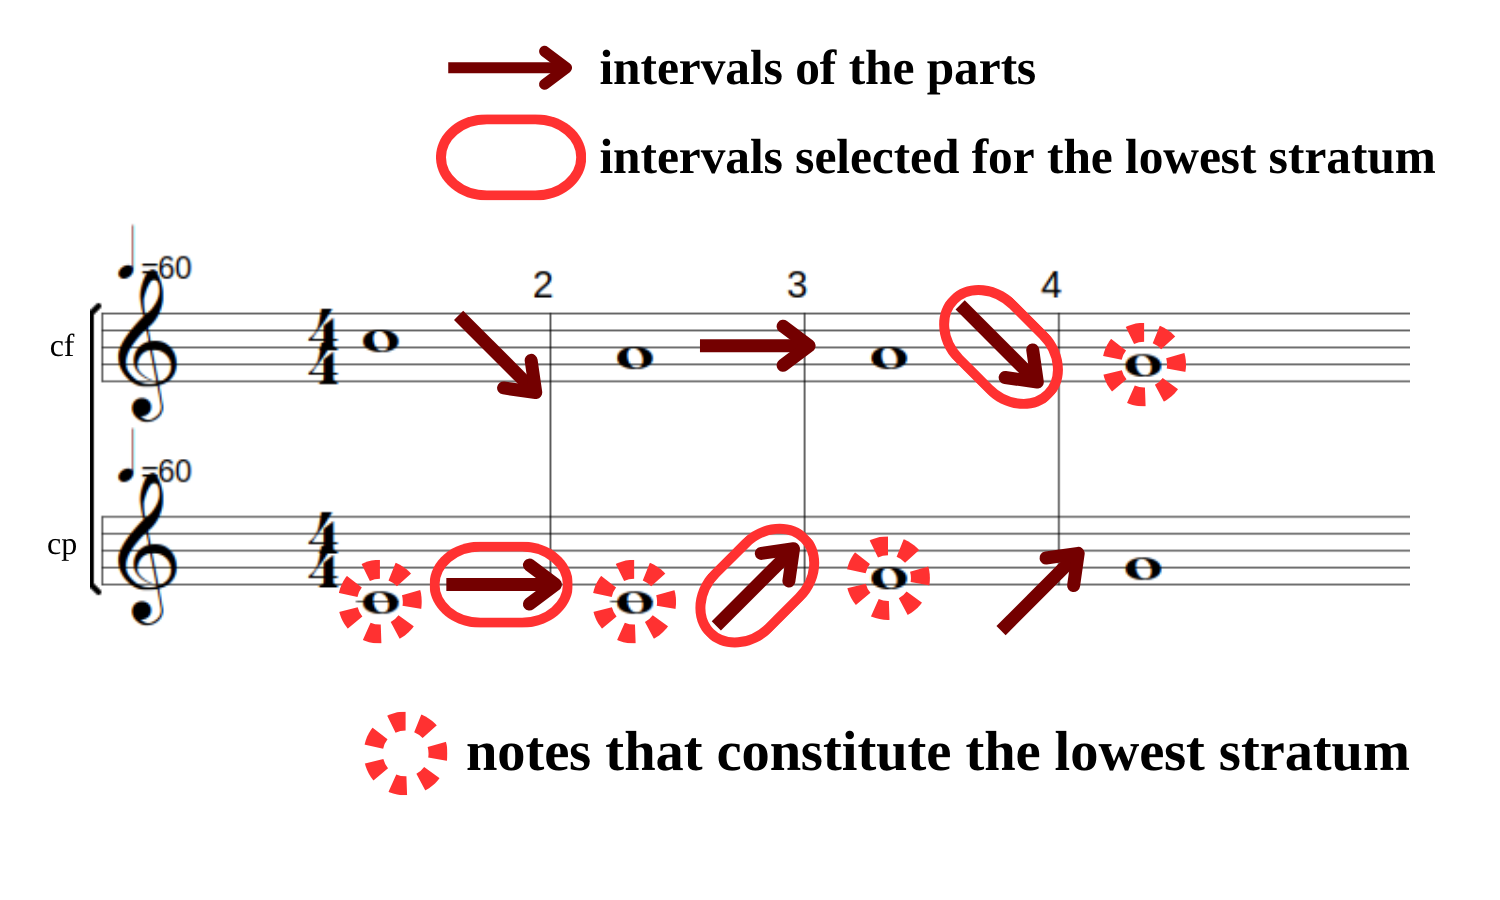
\includegraphics[width=\textwidth]{Images/stratum-m-intervals.png}
    \captionof{figure}{Understanding the melodic intervals of the lowest stratum with a first species counterpoint}
    \label{fig:stratum-m-intervals-1}
    \end{minipage}
    \hfill
    \begin{minipage}{0.46\textwidth}
      \centering
      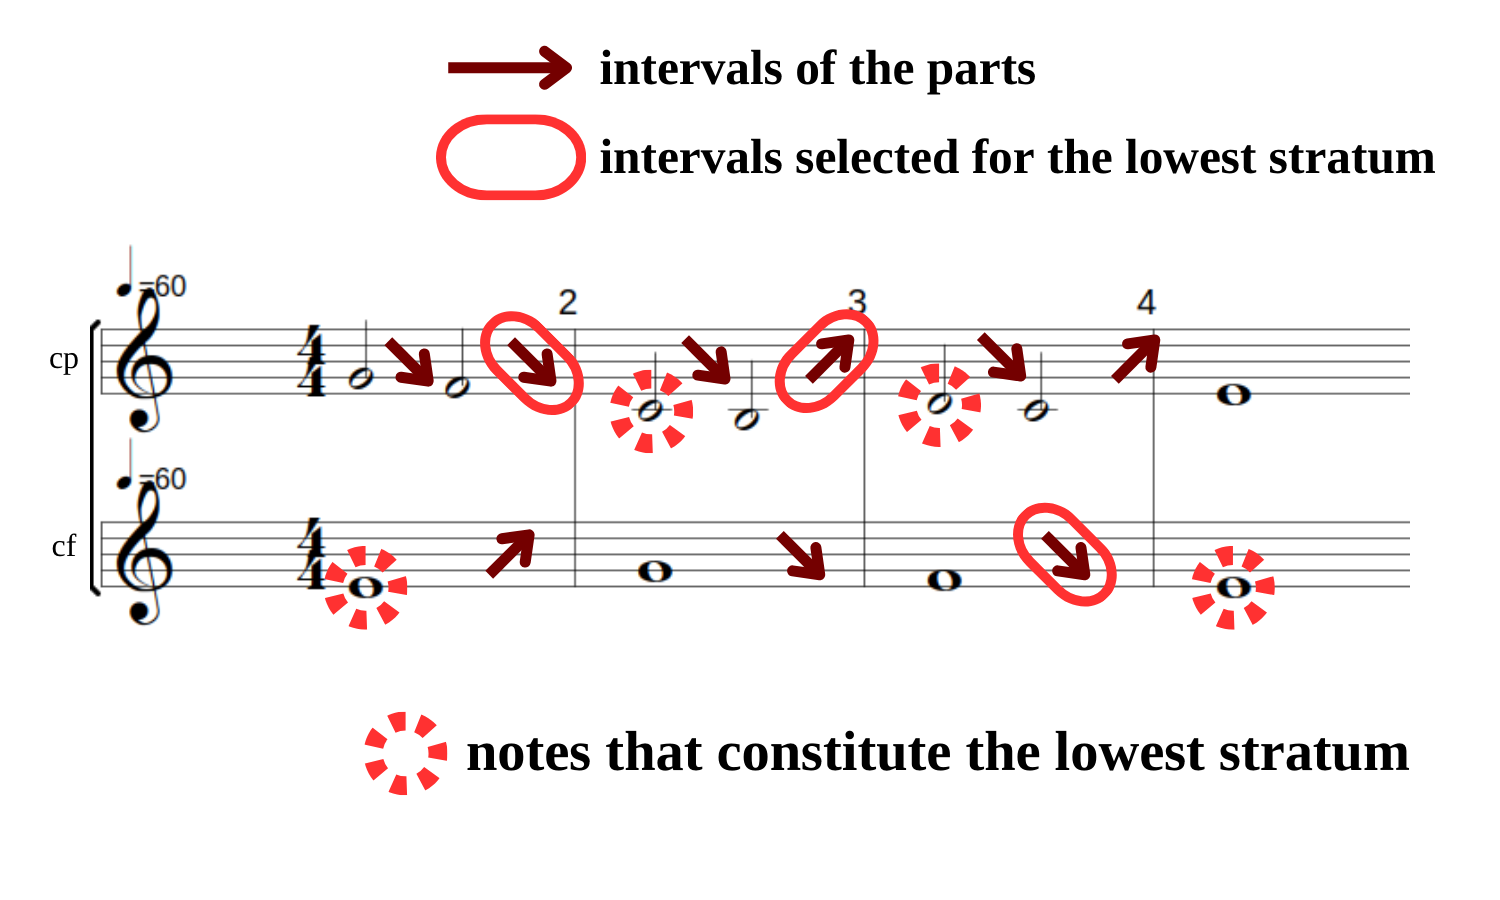
\includegraphics[width=\textwidth]{Images/stratum-m-intervals2.png}
      \captionof{figure}{Understanding the melodic intervals of the lowest stratum with a second species counterpoint}
      \label{fig:stratum-m-intervals-2}
\end{minipage}

\vspace{.5cm}
\noindent \textbf{P}(p) \hspace*{.2cm} \texttt{motions}

The motions array represents the motions\footnote{Reminder: there are three types of motion: direct, when both voices move together, contrary, when one voice moves up and the other moves down, and oblique, when one voice doesn't move and the other does} of a part p with respect to the lowest stratum. Of course, to be able to compute the motions between two voices, we must compare their melodic intervals, hence, we must deal with melodic intervals of a stratum. This is not a problem anymore since we have defined what the melodic intervals of the lowest stratum mean in the previous sub-section.
However, a problem arises when computing the motions of the part that is also the lowest stratum in some measures. When this happens, we end up calculating motions between a part and itself. Any part is inevitably moving in direct motion with itself, and this situation leads to only direct motions being calculated. This becomes problematic when considering costs (it is bad to have direct motions, but it obviously should not be bad to be the lowest stratum), and when considering some constraints. To tackle this problem, the motions of a part are now equal to -1 when the part is also the lowest stratum (which is denoted A(p), see section~\ref{is-lowest}). This value can be considered as a 'non-applicable' value: this part has no motion as it is currently the lowest stratum.

\begin{equation}
\begin{aligned}
&\forall p \in \{\mathit{cf}, cp_1, cp_2\}, \quad \forall x \in \{1, 2\}, \quad \forall i \in B, \quad \forall j \in [0, m - 1),\quad x := b - i\\
    &motion(p)[i,j] = \,  
    \begin{cases}
        0 &\text{if } (M_{brut}^{x}(p)[i, j] > 0 > M(a)_{brut}[j]) \\ & \quad \quad \quad \quad \quad \quad \quad \quad \quad  \vee (M_{brut}^{x}(p)[i, j] < 0 < M(a)_{brut}[j]) \\
        &\\
        1 &\text{if } M_{brut}^{x}(p)[i, j] = 0  \oplus M(a)_{brut}[j]=0 \\
        &\\
        2 &\text{if } (M_{brut}^{x}(p)[i, j] > 0 \land M(a)_{brut}[j] > 0) \\ & \quad \quad \quad \quad \quad \quad \quad \quad \quad   \vee  (M_{brut}^{x}(p)[i, j] < 0 \land M(a)_{brut}[j] <0)\\
        &\quad \quad \quad \quad \quad \quad \quad \quad \quad \vee (M_{brut}^{x}(p)[i, j] = 0 = M(a)_{brut}[j])
    \end{cases} 
    \\
    &P(p)[i,j] = \,  
    \begin{cases}
        -1 & \text{if } A(p)[j] \\
        motion(p)[i,j] & \text{if } \neg A(p)[j]
    \end{cases}
\end{aligned}
\label{eq:motions}
\end{equation}

This equation~\ref{eq:motions} may seem daunting, but it's actually very simple (just a little verbose).
It works like this: 

For each beat in the composition:
\begin{itemize}
    \item If a part is also the lowest stratum, P is -1 (i.e. non applicable, otherwise we would calculate the motion between the part and itself).
    \item If the part moves in the opposite direction to the lowest stratum, P is 0.
    \item If the part stays where it is and the lowest stratum moves (or vice versa), P is 1.
    \item If the part moves in the same direction as the lowest stratum, P is 2.
\end{itemize}

\vspace{.5cm} \noindent \textbf{A}(p) \hspace{.cm} \texttt{is-lowest} \label{is-lowest}
% expliquer en EN que on peut pas lambda(cp1) ET lambda(cf)

A is an array of boolean variables with a size of $m$ (the number of measures), where each variable indicates whether the corresponding part is the lowest stratum. In other words, $A(p)$ is true if p is the lowest stratum. The notation "A" was chosen as the uppercase of "a", which itself represents the lowest stratum. 
It is also worth to be noted that only one of the parts can be the lowest stratum at the time. This does not mean that two parts cannot equal the lowest stratum at the same time, it \textit{is} indeed possible that two parts blend in unison in the final chord, and that both pitches are the lowest sounding notes. It means that only one of those two is going to be considered to \textit{be} the lowest stratum (and the other one will be the intermediate stratum). This is needed in order for motions to work well, see~\ref{subsubsection:one-part-per-stratum} for the details.

Here is the mathematical definition of the A array:
\begin{equation}
\begin{aligned}
\forall j \in [0, m)& \colon  \\
A(\mathit{cf})[j] &= \,  
\begin{cases}
    \top & \text{if } N(cf)[0,j] = N(a)[0,j] \\
    \bot & \text{else }
\end{cases}\\
A(cp_1)[j] &= \,  
\begin{cases}
    \top & \text{if } (N(cp_1)[0,j] = N(a)[0,j]) \land \neg A(\mathit{cf})[j] \\
    \bot & \text{else }
\end{cases}\\
A(cp_2)[j] &= \,  
\begin{cases}
    \top & \text{if } \neg A(\mathit{cf}) \land \neg A(cp_1)\\
    \bot & \text{else }
\end{cases}
\end{aligned}
\end{equation}

As can be seen in these equations, only the downbeat of each measure is taken into account when computing the A array. The reason for this is that it is the downbeat note that determines which chord will be \textit{the} chord of the measure, and the other beats are just fioritures. Another reason for this is also that it is only going to serve in contexts where the first note of the measure is relevant.

\paragraph{}
In practice, there is only an \texttt{is-not-bass} array in the code (which is then equal to $\neg A$), as it is almost always more useful to know if a part is \textit{not} the lowest stratum than knowing if it is the lowest one. 

